\section{Lecture 1. Introduction and Basic DP Algorithm}
\subsection{Basic Strucutre of Stochastic DP}
\begin{itemize}
    \item 2 principle features of DP
        \begin{itemize}
            \item Discrete-time dynamic system
            \item Cost function is additive over time
        \end{itemize}
    \item 6 key elements of DP formulation
        \begin{itemize}
            \item \textbf{Stage}: $k$
            \begin{itemize}
                \item Finite horizon. Total number of horizon: $N$.
            \end{itemize}
            \item \textbf{State}: $x_k$
            \item \textbf{Control}: $u_k\in U_k(x_k)$ (or called \textbf{Decision, Action})
            \item \textbf{Disturbance}: $w_k$
            \item \textbf{"Memoryless" System Dynamics}: $x_{k+1}=f_k(x_k,u_k,w_k)$
                \begin{itemize}
                    \item Alternative system equation: $P(x_{k+1}|x_k,u_k)$
                \end{itemize}
            \item \textbf{"Additive" Stage Cost}: $g_k(x_k,u_k,w_k)$
                \begin{itemize}
                    \item Terminal Stage Cost: $g_N(x_N)$
                    \item Total cost: $\mathbb{E}_{w_0,w_{k-1}}\{g_N(x_N)+\sum_{k=0}^{N-1}g_k(x_k,u_k,w_k)\}$
                \end{itemize}
        \end{itemize}
    \item Additional Assumptions
        \begin{itemize}
            \item The feasible set of $u_k$, $U_k(x_k)$, depends at most $x_k$ and not on prior $x$ or $u$.
            \item The probability distribution of $w_k$ may depends on $x_k,u_k$ but not past values $w_0,...,w_{k-1}$.
                \begin{itemize}
                    \item $P(w_k|x_k,u_k)$
                \end{itemize}
            \item [] \emph{This two assumptions ensures the optimization of $u_k$ only requires the information of $x_k$ and $u_k$, which is "Memoryless". 
            Past values of $x$ or $w$ should be useless for future optimization.}
        \end{itemize}
    \item Sequence of events envisioned in period $k$: \\
    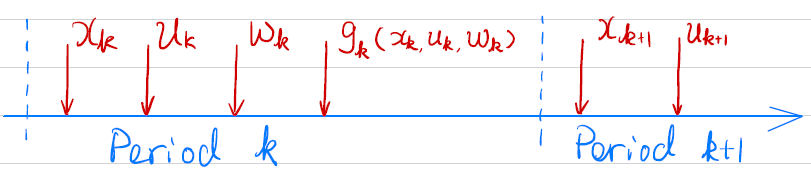
\includegraphics[width=15cm]{Lecture1/Fig1.png}
        \newpage
        \begin{itemize}
            \item $x_k$ occurs according to system dynamics
                \begin{itemize}
                    \item $x_k=f_{k-1}(x_{k-1},u_{k-1},w_{k-1})$
                \end{itemize}
            \item $u_k$ is selected with knowledge of $x_k$
                \begin{itemize}
                    \item $u_k\in U_k(x_k)$
                \end{itemize}
            \item $w_k$ is random and generated according to a distribution
                \begin{itemize}
                    \item $w_k ~ P(w_k|x_k,u_k)$
                \end{itemize}
            \item $g_k(x_k,u_k,w_k)$ is incurred and added to previous costs
        \end{itemize}
    \item Basic problem
        \begin{itemize}
            \item \textbf{Policies} $\pi=\{\mu_0,...,\mu_{N-1}\}$
                \begin{itemize}
                    \item $\mu_k$ maps states $x_k$ into controls $u_k=\mu_k(x_k)$
                    \item $\mu_k(x_k)\in U_k(x_k)$ for all $x_k$
                \end{itemize}
            \item \textbf{Expected cost} of policy $\pi$ starting at $x_0$ is
                \begin{itemize}
                    \item $J_{\pi}(x_0)=\mathbb{E}\{g_N(x_N)+\sum_{k=0}^{N-1}g_k(x_k,\mu_k(x_k),w_k)\}$
                \end{itemize}
            \item \textbf{Optimal cost function}
                \begin{itemize}
                    \item $J^*(x_0)=\min_{\pi}J_\pi(x_0)$
                \end{itemize}
            \item \textbf{Optimal policy} $\pi^*$
                \begin{itemize}
                    \item $J_{\pi^*}(x_0)=J^*(x_0)$
                \end{itemize}
        \end{itemize}
    \item 2 aims
        \begin{itemize}
            \item \textbf{Optimal policy} 
                \begin{itemize}
                    \item $u_k=\mu_k^*(x_k)$ for all $k=1,...,N-1$
                    \item $\pi^*=(\mu_0^*,\mu_1^*,...,\mu_{N-1}^*)$
                \end{itemize}
            \item \textbf{Value function}
            \begin{itemize}
                \item $J_N(x_N)=g_N(x_N)$
                \item $J_k(x_k)= \underset{u_k\in U_k(x_k)}{\min} \mathbb{E}_{w_k}\{g_k(x_k,u_k,w_k)+J_{k+1}(f_k(x_k,u_k,w_k))\}$, $\forall k=0,1,...,N-1$ \\
            \end{itemize}
        \end{itemize}
\end{itemize}

\newpage
\subsection{Example 1. Inventory Control}
\begin{itemize}
    \item \textbf{Stage}: Ordering period $k$
    \item \textbf{State}: Inventory level at period $k$, $x_k$
    \item \textbf{Control}: Sotck ordered at period $k$, $u_k\geq 0$
    \item \textbf{Disturbance}: Demand at period $k$, $w_k$
    \item \textbf{System Dynamics}: $x_{k+1}=f_k(x_k,u_k,w_k)=x_k+u_k-w_k$
    \item \textbf{Stage Cost}: $g_k(x_k,u_k,w_k)= \underbrace{k\cdot \mathbbm{1}_{[u_k>0]}}_{\textbf{\rm Set up}} + \underbrace{c\cdot u_k}_{\textbf{\rm Ordering fee}} + \underbrace{h(x_k+u_k-w_k)^{+}}_{\textbf{\rm Holding cost}}  + \underbrace{p(x_k+u_k-w_k)^{-}}_{\textbf{\rm Shortage penalty}}$
    \item \textbf{Terminal Cost}: $g_N(x_N)=0$
\end{itemize}

\subsection{Example 2. Scheduling}
\begin{itemize}
    \item Find the optimal sequence of operations $A,B,C,D$
    \item $A$ must precede $B$, $C$ must precede $D$
    \item Given startup cost $S_A,S_C$ and setup transition cost $C_{nm}$ from operation $m$ to $n$
    \item This is a \textbf{Deterministic Finite-State Problem}.
\end{itemize}
\centerline{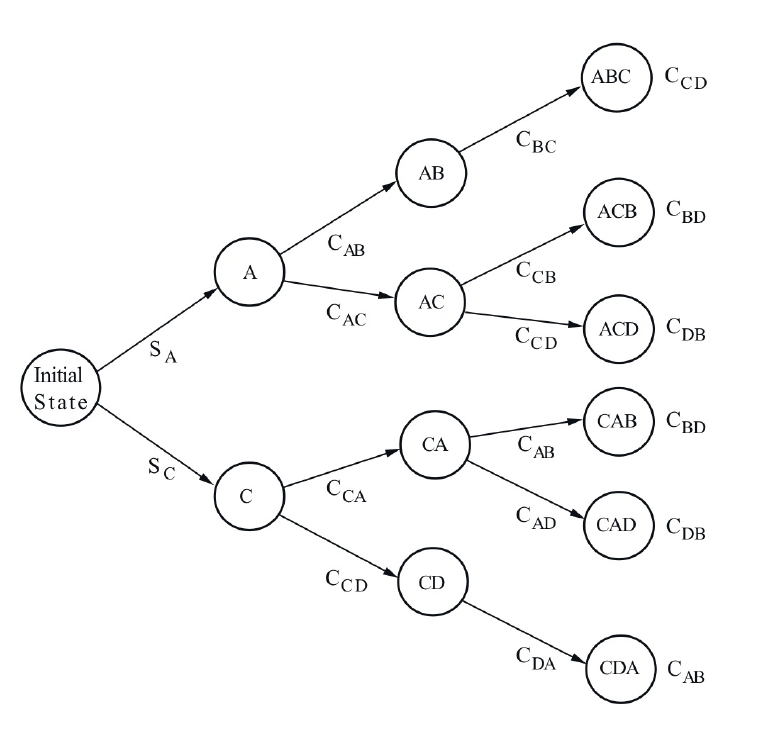
\includegraphics[width=12cm]{Lecture1/Fig2.png}}

\subsection{Example 3. Two-game Chess}
\begin{itemize}
    \item Find two-game chess match strategy
    \item \textbf{State}: Match score
    \item \textbf{Control}: Timid play \emph{or} Bold play
    \item \textbf{System Dynamics}:
        \begin{itemize}
            \item Timid play: draws with $P_d>0$ and loses with $1-P_d$
            \item Bold play: wins with $P_w\leq \frac{1}{2}$ and loses with $1-P_w$
        \end{itemize}
    \item \textbf{Value of information} = $J^*_{\textbf{\rm closed-loop}} - J^*_{\textbf{\rm open-loop}}$
        \begin{itemize}
            \item Open-loop policy: play always Bold
            \item Close-loop policy: Play Timid if and only if you are ahead
        \end{itemize}
    \emph{See the example in Apendix.1}
\end{itemize}

\subsection{Principle of Optimality}
\begin{itemize}
    \item Consider the \textbf{"tail subproblem"}. Minimize the "cost-to-go" from $i$ to $N$
        \begin{itemize}
            \item $\mathbb{E}\{g_N(x_N)+\sum_{k=1}^{N-1}g_k(x_k,\mu_k(x_k),w_k)\}$
        \end{itemize} 
    \item Consider the \textbf{"tail policy"}
        \begin{itemize}
            \item $\{\mu_i^*,\mu_{i+1}^*,...,\mu_{N-1}^*\}$
        \end{itemize} 
    \item \textbf{Principle of optimality}: The tail policy is optimal for the tail subproblem.
    \item DP first solve ALL tail subproblems of final stage
    \item At the generic step, DP solves ALL tail subproblems of a given time length, using the solution of the subproblems of shorter length
\end{itemize}

\subsection{Demonstration for the Principle of Optimality (Inventory Control)}
\begin{itemize}
    \item $J_N(x_N) = 0$
    \item Tail subproblem of length 1 ($u_{N-1}=\mu_{N-1}^*(x_{N-1})$)
    \[
        \begin{array}{ll}
            J_{N-1}(x_{N-1})    &= \min_{u_{N-1}\geq 0} \mathbb{E}_{w_{N-1}}\{ cu_{N-1} + r(x_{N-1}) + u_{N-1} - w_{N-1} + J_N(x_{N-1}+u_{N-1}-w_{N-1}) \} \\
                                &= \min_{u_{N-1}\geq 0} \mathbb{E}_{w_{N-1}}\{ cu_{N-1} + r(x_{N-1}) + u_{N-1} - w_{N-1}) \}
        \end{array}
    \]
    \item Tail subproblem of length $N-k$ ($u_{k}=\mu_{k}^*(x_{k})$)
    \[
        J_{k}(x_{k}) = \min_{u_{k}\geq 0} \mathbb{E}_{w_{k}}\{ cu_{k} + r(x_{k}) + u_{k} - w_{k} + J_{k+1}(x_{k}+u_{k}-w_{k}) \}
    \]
    \item $J_0(x_0)$ is the optimal cost of initial state $x_0$
\end{itemize}

\subsection{DP Algorithm}
Original Problem:
\[
    \begin{array}{ll}
        J^*(x_0) =  & \min_{x\in\pi} J_\pi(x_0) = \min_{x\in\pi} \mathbb{E} \left\{ g_N(x_N) + \sum_{k=0}^{N-1} g_k(x_k,\mu_k(x_k),w_k) \right\} \\
                    &\text{\rm s.t. } x_{k+1} = f_k(x_k,\mu_k(x_k),w_k) \\
                    &\text{\rm where } \pi = \{ \mu_0,\mu_1,...,\mu_{N-1} \}
    \end{array}
\]
DP algorithm:
\begin{itemize}
    \item Start with $J_N(x_N)=g_N(x_N)$ and go backwards using
    \[
        J_k(x_k) = \min_{u_k\in U_k(x_k)} \mathbb{E}_{w_k} \{ g_k(x_k,u_k,w_k) + J_{k+1}\left( f_k(x_k,u_k,w_k) \right) \}\quad , k=0,1,...,N-1
    \]
    This means that $u_k=\mu^*_k(x_k)$.
    \item Then $J_0(x_0)$, generated at the last setp, is equal to the optimal cost $J^*(x_0)$. \\ Also, the policy $\pi^*=\{\mu_0^*,...,\mu_{N-1}^*\}$.
\end{itemize}
Some remark:
\begin{itemize}
    \item Ideally, the DP algorithm can be used to obtain closed-form expressions for $J_k$, the cost-to-go function at $k$, or an optimal policy
    \item Even if models may rely on over-simplified assumption, they may provide valuable insights about the structures of the optimal solution of more complex models and form the basis for suboptimal control scheme
    \item Unfortunately, an analytical solution is not possible in many practical cases, and one has to resort to numerical execution of the DP algorithm
    \item DP is the only general approach for sequential optimization under uncertainty, and even when it is computationally prohibitive, it can serve as the basis for more practicval suboptimal approaches
\end{itemize}
[Example, Proof ...]

\subsection{State Augmentation}
\begin{itemize}
    \item When assumptions of the basic problem are violated (e.g., disturbances are correlated, cost is nonadditive, etc) reformulate/augment the state
    \item DP algorithm still applies, but the problem gets bigger
    \item \textbf{Example}: \\Time lags
    \[
        x_{k+1} = f_k(x_k,x_{k-1},u_k,w_k)
    \]
    \[
        x_1 = f_0(x_0,u_0,w_0)
    \]
    \begin{itemize}
        \item Introduce additional state variable $y_k=x_{k-1}$. New system takes the form
        \[
            \left(\begin{array}{cc} x_{k+1} \\ y_{k+1} \end{array}\right) = \left(\begin{array}{cc} f_k(x_k,y_k, u_k,w_k) \\ x_k \end{array}\right)
        \]
        View $\tilde{x}_k = (x_k,y_k)$ as the new state.
        \item DP algorithm for the formulated problem:
        \[
            J_k(x_k,x_{k-1}) = \min_{u_k\in U_k(x_k)} \mathbb{E}_{w_k} \{g_k(x_k,u_k,w_k) + J_{k+1}(f_k(x_k,x_{k-1}, u_k,w_k),x_k)\}
        \]
    \end{itemize}
    \item \textbf{Example}: \\Correlated disturbances
    \[
        w_k = \lambda w_k + \xi _k
    \]
    \begin{itemize}
        \item Let $y_k=w_{k-1}$
        \[
            \tilde{x}_{k+1} = \left(\begin{array}{cc} x_{k+1} \\ y_{k+1} \end{array}\right) = \left(\begin{array}{cc} f_k(x_k,u_k,\lambda y_k + \xi_k) \\ \lambda y_k + \xi_k \end{array}\right)
        \]
        View $\tilde{x}_k = (x_k,y_k)$ as the new state.
        \item DP algorithm for the formulated problem:
        \[
            J_k(x_k,y_k) = \min_{u_k\in U_k(x_k)} \mathbb{E}_{\xi_k} \{g_k(x_k,u_k,\lambda y_k + \xi_k) + J_{k+1}(f_k(x_k,u_k,\lambda y_k + \xi_k),\lambda y_k + \xi_k)\}
        \]
    \end{itemize}
\end{itemize}